\chapter{APRENDIZAJE AUTOMÁTICO}\label{chp:Teoria}%Diseño Teórico
En este capítulo se abordarán conceptos importantes sobre aprendizaje automático, el aprendizaje profundo, el funcionamiento y las características de estas áreas de estudio.



\section{GENERALIDADES}
Para definir el concepto de aprendizaje automático con una buena perspectiva, debemos, primeramente definir qué es la inteligencia artificial. 

La inteligencia artificial en un enfoque de actuar humano se define como ``El arte de crear máquinas que realicen funciones que requieren inteligencia cuando las realizan personas''.\cite[p. 2]{stuart2010artificial}. De esta rama de la informática han surgido campos que actualmente están siendo potencialmente estudiados como: el procesamiento del lenguaje natural, el aprendizaje automático, el aprendizaje profundo, la visión por computadora, etc.

Los avances en estas áreas de estudio han dado como resultado aplicaciones populares, tales como: modelos de clasificación de texto, modelos de traducción de idiomas, cualquier modelo generativo, sistemas de conducción autónomos de vehículos, etc.

Muchos de estos sistemas y aplicaciones inteligentes son parte de una vida diaria, donde probablemente se usen de manera desapercibida, se podría decir que ha surgido la nueva fiebre por la inteligencia artificial. Nunca antes como ahora la inteligencia artificial había sido tan nombrada en noticias, medios de comunicación o revistas científicas, y tan ampliamente usada por cualquiera que así lo necesite, tenga o no conocimiento técnico de esta rama de estudio. Una de las razones sobre la que descansa toda esta popularidad es el aprendizaje automático.

El aprendizaje automático se enfoca en la creación de algoritmos y modelos que permiten a las máquinas aprender patrones a partir de una gran cantidad de datos, capacitándolas para llevar a cabo tareas específicas sin necesidad de seguir instrucciones programadas.

Arthur Samuel, en 1959, definió el aprendizaje automático como: ``El campo de estudio que otorga a las computadoras la capacidad de aprender sin ser programadas explícitamente'' \cite[p. 281]{geron2019hands}.

Posteriormente, en 1997, Tom Mitchell proporcionó otra definición clave: ``Se dice que un programa de computadora aprende de la experiencia E con respecto a alguna tarea T y alguna medida de desempeño P, si su desempeño en T, medido por P, mejora con la experiencia E''\cite[p. 281]{geron2019hands}.

En el campo del aprendizaje automático, se encuentran algoritmos fundamentales que son comúnmente empleados en tareas relacionadas con texto, algunos de estos son: la regresión logística, los árboles de decisión y Naive Bayes. Estos algoritmos tienen notables limitaciones en cuanto a su capacidad para aprender representaciones jerárquicas de texto, captura de contexto, modelar relaciones no lineales y escalar eficazmente. Pero en casos donde el conjunto de datos es reducido y la tarea no implica complejidades profundas en el análisis de características del texto, estos modelos más simples pueden mostrar un rendimiento satisfactorio.

Ya que se menciona al conjunto de datos necesario para entrenar estos y otros algoritmos de aprendizaje es importante aclarar que uno de los desafíos del aprendizaje automático radica en la recopilación de datos. Lo ideal sería contar con miles de millones de datos que se encuentren balanceados, limpios, etiquetados y que además sean representantes valiosos para la tarea a realizar. Sin embargo esta situación es casi imposible de alcanzar. Encontrar conjuntos de datos más o menos adecuados para alguna tarea ya puede considerarse un éxito y un gran avance para el proyecto. Sin embargo, si no se obtiene siquiera esa ventaja, debe procederse a una exhaustiva recopilación de datos que además implica un riguroso proceso de revisión, limpieza, análisis, preprocesamiento, etiquetado y muchas otras tareas más.

\begin{figure}
	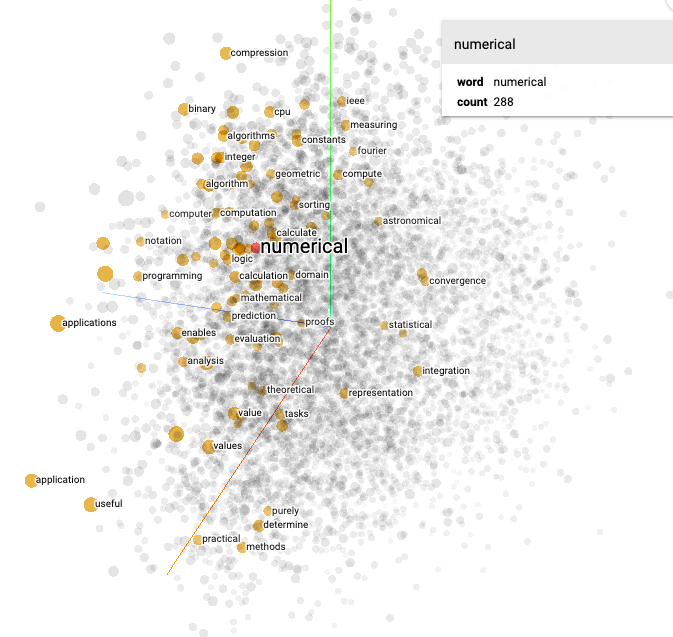
\includegraphics[width=0.65\textwidth]{capitulo2/figuras/an1.png}
	\caption{Representacion vectorial tridimensional de incrustaciones de palabras en TensorBoard}
	\floatfoot{Fuente: Elaboracion propia utilizando TensorBoard }
	\label{fig:tensorboard}
\end{figure}

Uno de los subcampos fundamentales del aprendizaje automático, que depende en gran medida de la calidad y cantidad de los datos, es el aprendizaje profundo. El aprendizaje profundo se centra en el entrenamiento de redes neuronales con múltiples capas apiladas, cada una compuesta por neuronas interconectadas que realizan operaciones matemáticas con los datos.

La diferencia principal entre las redes neuronales tradicionales y las redes neuronales profundas radica en la capacidad de estas últimas para comprender características complejas de los datos. Un ejemplo notable de esta capacidad se evidencia en modelos de aprendizaje profundo como Word2Vec, cuya función es representar palabras como vectores densos.\\
Word2Vec tiene en cuenta el contexto en el que aparecen las palabras, lo que facilita la captura de significados contextualmente relevantes. En la Figura \ref{fig:tensorboard}  se puede observar una representación de embeddings de 10,000 palabras en la interfaz de Tensorflow. Con el vector de la palabra ``numerical'' como punto de referencia, se pueden observar los vectores de las palabras más cercanos a numerical que, resaltan ya sea por contexto, sintaxis o similitud semántica. El cálculo de estas características complejas sólo puede llevarse a cabo mediante redes de aprendizaje profundo. 

Esta breve introducción tiene como objetivo dar una perspectiva amplia sobre estos conceptos fundamentales con algunos ejemplos que permitan comprender las aplicaciones del aprendizaje automático y profundo. En las siguientes secciones del capítulo se realizará una exploración más profunda sobre el funcionamiento, las ventajas y limitaciones de estas dos áreas de estudio.



\section{NEURONAS BIOLÓGICAS VS NEURONAS ARTIFICIALES}
A continuación se presentan trabajos relevantes que han contribuido a la representación de la neurona, sentando las bases de los modelos neuronales actuales. Además, se explora en detalle el funcionamiento y las características de una neurona artificial, tal como se conoce comúnmente en la actualidad.
\subsection{ Modelo neuronal de Warren McCulloch y Walter Pitts}
Uno de los trabajos más relevantes sobre la representación de una neurona biológica fue el de Warren McCulloch y Walter Pitts quienes se consideran  pioneros en el campo de las neurociencias computacionales y la teoría de las redes neuronales artificiales. En 1943, publicaron un artículo titulado ``A Logical Calculus of Ideas Immanent in Nervous Activity'' (``Un cálculo lógico de ideas inmanentes en la actividad nerviosa''), donde presentaron un modelo muy simplificado de una neurona biológica, que es considerado uno de los primeros modelos de neuronas artificiales\cite{mcculloch1943logical}.

\begin{figure}
	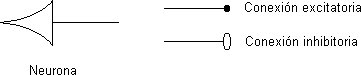
\includegraphics[width=0.65\textwidth]{capitulo2/figuras/an2.png}
	\caption{Representacion grafica de una neurona y sus dos tipos de conexiones}
	\floatfoot{Fuente: El modelo neuronal de McCulloch y Pitts: Interpretacion comparativa del modelo \cite[ p.4]{prieto2020modelo} }
	\label{fig:an2}
\end{figure}

Este modelo propuesto  fue una abstracción matemática de cómo funciona una neurona biológica, y fue formulado como un sistema de lógica binaria. En su modelo, una neurona recibe múltiples señales de entrada (excitatorias o inhibitorias) y produce una única salida binaria basada en una función umbral. Si la suma de las señales de entrada superaba un cierto umbral, la neurona se activaba y emitía una señal de salida, de lo contrario, permanecía inactiva.

\begin{figure}[h!]
	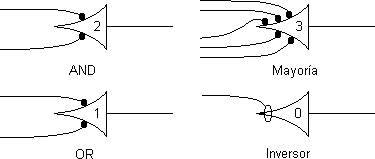
\includegraphics[width=0.65\textwidth]{capitulo2/figuras/an3.png}
	\caption{Algunos ejemplos de la implantacion de funciones logicas}
	\floatfoot{Fuente: El modelo neuronal de McCulloch y Pitts: Interpretacion comparativa del modelo \cite[p. 5]{prieto2020modelo} }
	\label{fig:an3}
\end{figure}

Aunque este modelo es muy simple en comparación con la complejidad de las neuronas biológicas reales, sentó las bases para el desarrollo de redes neuronales artificiales, esto debido a que ellos podían darnos a entender que la resolución de problemas más complejos  podría ser posible con la  conexión de muchas de estas neuronas. En la Figura \ref{fig:an2} se puede observar la representación básica de una neurona interpretando al modelo de Warren McCulloch y Walter Pitts , donde se aborda y representa los conceptos de conexión excitatoria e inhibitoria, que es equivalente a la sinapsis excitatoria e inhibitoria de una neurona biológica. En la Figura \ref{fig:an3} en la esquina superior izquierda se puede observar a la representación de una neurona cuyo funcionamiento es equivalente a una compuerta and de dos entradas, en la esquina inferior izquierda se encuentra otra neurona que es equivalente a una compuerta or de dos entradas , en la esquina superior derecha se aprecia a una neurona or de 5 entradas con un umbral de tres y finalmente en la esquina inferior derecha se observa una neurona con una  conexión inhibitoria con umbral cero.






\subsection{Perceptrón de clasificación binaria}
El perceptrón es un modelo de neurona artificial llamada unidad lógica de umbral (TLU, por sus siglas en inglés: Threshold Logic Unit) , desarrollado por Frank Rosenblatt en 1957. Es un modelo simple, donde una única neurona puede ser utilizada para problemas de clasificación binaria \cite{rosenblatt1957perceptron}.

El perceptrón es un caso particular y simple, con una función de activación específica y aplicable principalmente a problemas lineales. “En el caso del perceptrón, la elección de la función de activación de signo está motivada por el hecho de que es necesario predecir una etiqueta de clase binaria” \cite[p. 11]{aggarwal2018neural}. Esta función de activación suele ser una función escalón, produciendo una salida binaria (0 o 1).  Por lo tanto se utiliza para problemas de clasificación linealmente separables, lo que significa que solo puede resolver problemas donde se puede trazar una línea o un hiperplano para separar claramente las clases en un espacio de características.

\begin{figure}
	
	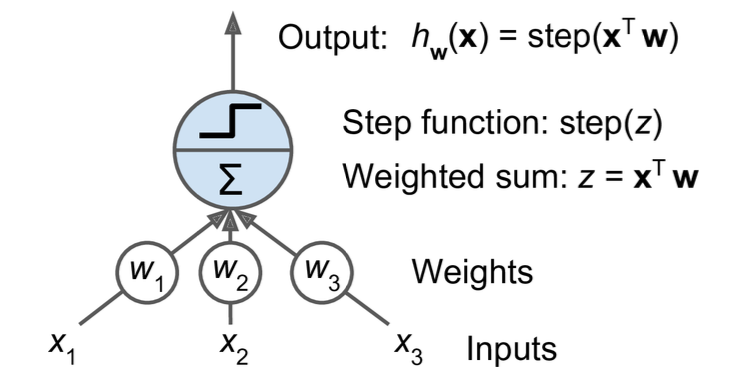
\includegraphics[width=0.65\textwidth]{capitulo2/figuras/an4.png}
	\caption{Unidad logica de umbral \\ \textit{Fuente:Extraido de \protect\cite[p. 282]{geron2019hands}}}
	\label{fig:an4}
\end{figure}

``El TLU calcula una combinación lineal de las entradas ( $\text{z} = w_1x_1 + w_2x_2 + \cdots + w_nx_n = x_Tw$) y si el resultado excede un umbral determinado en la función de paso , genera la clase positiva o genera la clase negativa''\cite[p. 282]{geron2019hands} ver Figura \ref{fig:an4}. 

La representación de una neurona artificial actual puede tener una función de activación más compleja que el escalón,  para permitir el aprendizaje en diferentes contextos. Por ejemplo, se puede emplear una función sigmoidal, tangente hiperbólica, ReLU, entre otras.







\subsection{Representación de una neurona artificial}
La comprensión actual de las neuronas artificiales, fundamentales en las redes neuronales del aprendizaje automático, se origina en la inspiración biológica y en modelos iniciales como los de Warren McCulloch, Walter Pitts y Frank Rosenblat . 

\begin{figure}[h!]
	\centering
	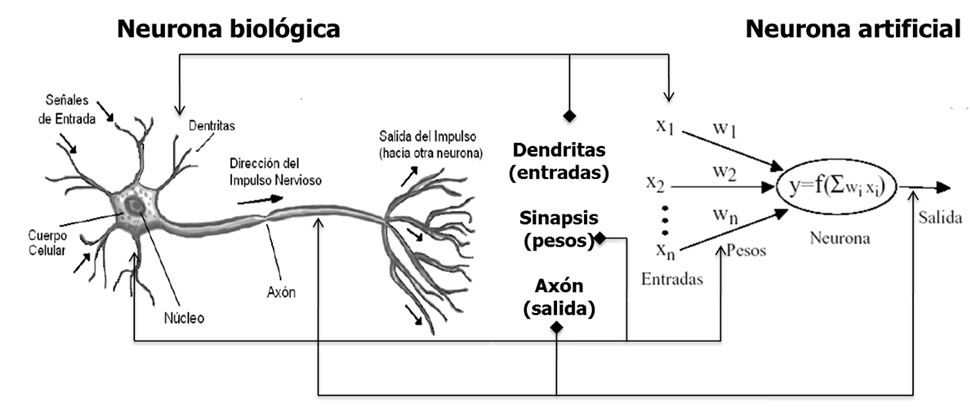
\includegraphics[width=0.65\textwidth]{capitulo2/figuras/an5.png}
	\caption{Comparación entre una neurona biológica y  artificial \\ \textit{Fuente: Extraido de \protect\cite[p. 4]{lao2017procedimiento}}}
	\label{fig:an5}

\end{figure}


El enfoque de McCulloch y Pitts representaba la neurona más  o menos como una compuerta lógica, la representación actual de la neurona en el contexto de las redes neuronales muestra una mayor complejidad y una aproximación más fiel a las funciones y comportamientos observados en el enfoque propuesto por Frank Rosenblatt. Este avance refleja un modelo más detallado y más cercano a la naturaleza multifacética y dinámica de las neuronas biológicas ver Figura \ref{fig:an5}.


Estructura Básica:
\begin{itemize}
	\item	 Neurona biológica: En el cerebro humano, las neuronas son células especializadas que forman la unidad básica del sistema nervioso. Tienen una estructura celular con un cuerpo celular, dendritas, axones y sinapsis.
	\item	Neurona artificial: En informática, una neurona artificial es la unidad básica de una red neuronal. Consiste en entradas, pesos, una función de activación y una salida.
\end{itemize}


Recepción y Transmisión de Señales:
\begin{itemize}
	\item	 Neurona biológica: Las dendritas reciben señales de otras neuronas a través de sinapsis. Cuando se acumula una cantidad suficiente de señales excitatorias o inhibitorias, se genera un impulso eléctrico a lo largo del axón hasta llegar a los botones sinápticos y posteriormente a la siguiente o siguientes neuronas, donde el proceso se repite nuevamente.
	\item	Neurona artificial: Recibe múltiples entradas que son multiplicadas por su respectivo peso, el peso que interviene en las entradas será lo suficientemente grande o pequeño para influir o no en la salida que posteriormente se modificará por alguna función de activación, debido a esta tarea es que la función de sinapsis de una neurona biológica es conceptualmente equivalente a la función de los pesos en una neurona artificial. 
\end{itemize}
Adaptabilidad y Aprendizaje:
\begin{itemize}
	\item	 Neurona biológica: Las neuronas biológicas pueden cambiar su conectividad y fuerza sináptica a lo largo del tiempo, lo que permite el aprendizaje y la adaptabilidad.
	\item	Neurona artificial: Los pesos en las neuronas artificiales pueden ajustarse durante el entrenamiento mediante algoritmos de aprendizaje, lo que permite que la red neuronal aprenda y mejore su capacidad para resolver tareas específicas.
\end{itemize}


\subsection{Función de entrada}
La función de entrada en una neurona artificial es el cálculo ponderado de las señales de entrada que recibe la neurona antes de aplicar una función de activación para producir la salida. En términos simples, la función de entrada representa cómo se combinan y procesan las entradas para determinar la actividad de la neurona.

En una neurona artificial básica, la función de entrada realiza alguna operación matemática conveniente, generalmente la suma de las señales de entrada multiplicadas por sus respectivos pesos. Esta suma ponderada se representa en la ecuación \ref{eq:e1}:

\begin{equation} \label{eq:e1} 
	Entrada = w_1x_1 + w_2x_2 + \cdots + w_nx_n + b 
\end{equation}

Donde : 
\begin{itemize}
\item $w_1, w_2, \ldots, w_n$ son los pesos asociados a cada señal de entrada $x_1, x_2, \ldots, x_n$ respectivamente.
\item $b$ es el sesgo (bias), un parametro adicional que se suma a la suma ponderada
\end{itemize}

\begin{figure}[h!]
	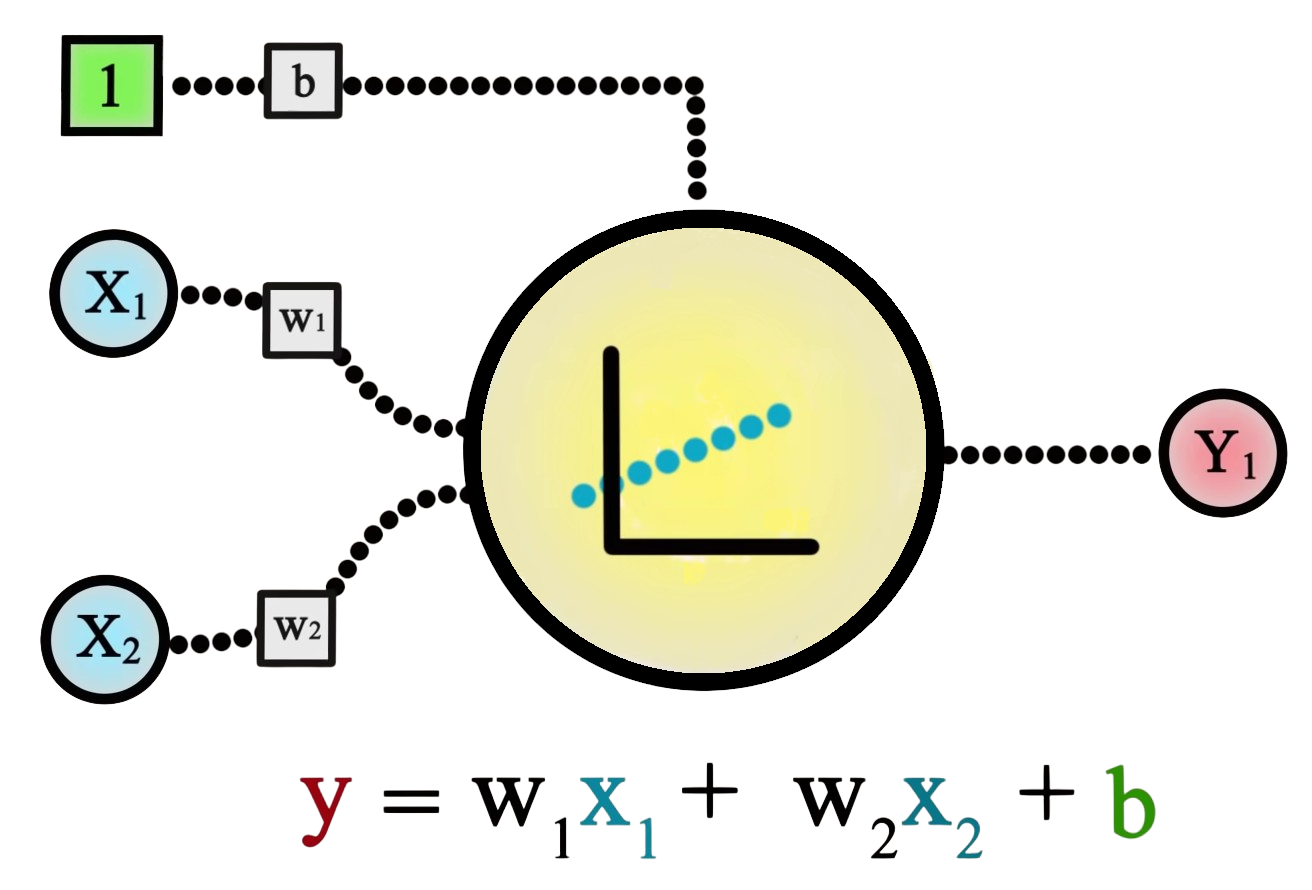
\includegraphics[width=0.65\textwidth]{capitulo2/figuras/an6.png}
	\caption[Representacion de una neurona artificial]{Representacion de una neurona artificial
		\\\textit{Fuente: Elaboracion Propia}}
	\label{fig:an6}
\end{figure}

Los pesos indican la importancia relativa de cada entrada en la determinación de la salida de la neurona, es decir, que permiten que un gran valor de entrada tenga solamente una pequeña influencia, si estos son lo suficientemente pequeños. El sesgo o bias es un término independiente que permite desplazar la función de entrada, lo que puede ser crucial para el aprendizaje y la adaptación de la red neuronal. Ver Figura \ref{fig:an6}. La función de entrada, en esencia, realiza un procesamiento lineal de las entradas ponderadas por sus pesos. Posteriormente, esta suma ponderada se introduce en una función de activación.


\subsection{Función de activación}
La función de activación es una función matemática no lineal que recibe las entradas procesadas de la neurona, se encarga de distorsionar el valor de salida, añadiendo valores no lineales. Ya que la neurona realiza generalmente una suma ponderada de sus entradas y esto puede asemejarse en esencia a un modelo lineal, para tratar problemas que no son solamente lineales se necesitan modelos más complejos, por lo tanto este es el propósito de una función de activación. ``Por ejemplo, si la variable objetivo que se va a predecir es real, entonces tiene sentido utilizar la función de activación de identidad y el algoritmo resultante es el mismo que el de la regresión de mínimos cuadrados.'' \cite[p. 11]{aggarwal2018neural}. Las funciones de activación más comúnmente utilizadas se detallan a continuación:


Función identidad: Es una función lineal que conserva el valor de entrada como salida, es la función más básica ya que no proporciona no linealidad:  Ver ecuación \ref{eq:e2}

\begin{equation} \label{eq:e2} 
	f(x) = x 
\end{equation}


	
Función sigmoide: Esta función tiene una forma de ``S'' y transforma la entrada a un rango de valores entre 0 y 1, esta característica facilita la interpretación como probabilidades, se alinea bien con modelos de máxima verosimilitud y permite la construcción de funciones de pérdida adecuadas para problemas de clasificación. Ver ecuación \ref{eq:e3}

\begin{equation} \label{eq:e3} 
	sigmoide(t)=\frac{1}{1+e^{-t}}
\end{equation}

 
	
	
Función tangente hiperbólica: Similar a la función sigmoide, pero tiene un rango entre -1 y 1. Es preferible a la sigmoide cuando se desea que los resultados de los cálculos sean tanto positivos como negativos. Su fórmula directa se puede observar en la ecuación \ref{eq:e4}.
 

\begin{equation} \label{eq:e4} 
tanh(x) = \frac{e^{x}-e^{-x}}{e^{x}+e^{-x}}
\end{equation}
	
Función tangente hiperbólica dura: La función ``hard tanh'' es una variante de la función tangente hiperbólica (tanh) que ha sido modificada para producir salidas en un rango limitado y discretizado, manteniendo las propiedades no lineales de la función tanh original pero restringiendo su rango de salida.
La función ``hard tanh'' es similar a la función tangente hiperbólica estándar, pero en lugar de proporcionar salidas en el rango continuo entre -1 y 1, aplica un límite a los valores de salida.

\begin{equation} \label{eq:e5} 
	hardTanh(x)=max(min(x,1), -1)
\end{equation}

	
	
Función ReLu: La función rectificada lineal se comporta de manera constante cuando el valor de z es menor a cero, o como una función lineal cuando el valor de z es mayor o igual a cero. ver ecuación \ref{eq:e6}

\begin{equation} \label{eq:e6} 
	relu(z)=max(0,z)
\end{equation}


Función softmax: Esta función transforma las salidas a una representación en forma de probabilidades, de tal manera que el sumatorio de todas las probabilidades de las salidas de uno. ver ecuación \ref{eq:e7}
\begin{equation} \label{eq:e7} 
	softmax(z_{j})=\frac{e^{z_{j}}}{\displaystyle\sum_{k=1}^{K}e^{z_{k}}}
\end{equation}




\subsection{ Función de salida}
La función de salida en una neurona artificial es la función que determina la salida final o el resultado de la neurona después de procesar las entradas y aplicar la función de activación. Esta función determina qué valor se transfiere a las neuronas vinculadas. ``Si la función de activación está por debajo de un umbral determinado, ninguna salida se pasa a la neurona subsiguiente.''\cite[p. 12]{matich2001redes} Normalmente, no cualquier valor es permitido como una entrada para una neurona. Algunos de los valores de salida pueden ser la salida misma o también pueden ser binarios {0, 1} o {-1, 1}.
\section{REDES NEURONALES}
En esta sección se detalla con más profundidad  acerca de los diversos conceptos de funcionamiento y arquitectura de redes neuronales.

\subsection{Redes neuronales feedforward}
Las redes neuronales feedforward, presentan una arquitectura donde la información fluye en una dirección única, avanzando desde la capa de entrada a través de una serie de capas ocultas hasta llegar a la capa de salida, sin ciclos ni retroalimentación. Por ejemplo, podemos visualizar este flujo como una sucesión de funciones $f_1(), f_2(), y f_3()$ encadenadas para formar $f(x) = f_3(f_2(f_1(x)))$. Estas estructuras en cadena son las formas más comunes de redes neuronales.

En esta secuencia, $f_1()$ representa la primera capa de la red, $f_2()$ sería la segunda capa, y así sucesivamente. La extensión total de esta cadena determina la profundidad del modelo. Este concepto de profundidad es esencial en la terminología del ``aprendizaje profundo'', un nombre derivado precisamente de esta característica.

Este enfoque, descrito en el libro Deep Learning \cite[p.167]{goodfellow2016deep}, permite representar y procesar datos de manera más compleja, ya que cada capa sucesiva puede aprender y extraer características más abstractas de los datos de entrada, posibilitando así la resolución de problemas complejos.

\subsection{Perceptrón multicapa}
El perceptrón multicapa, también conocido como red neuronal de múltiples capas es un ejemplo de red neuronal profunda feedforward, es una extensión del perceptrón simple que consta de múltiples capas de neuronas interconectadas, la representación gráfica de un perceptron multicapa con dos capas ocultas se puede observar en la figura \ref{fig:an7}. A diferencia del perceptrón de una sola capa, el perceptrón multicapa tiene al menos una capa oculta (capas entre la capa de entrada y la capa de salida), lo que le permite resolver problemas más complejos y no linealmente separables.

Esta red neuronal se entrena utilizando algoritmos de aprendizaje supervisado, como retropropagación (backpropagation), que ajustan los pesos de las conexiones entre las neuronas para minimizar una función de pérdida, mejorando así la capacidad de la red para hacer predicciones precisas.

\begin{figure}[h!]
	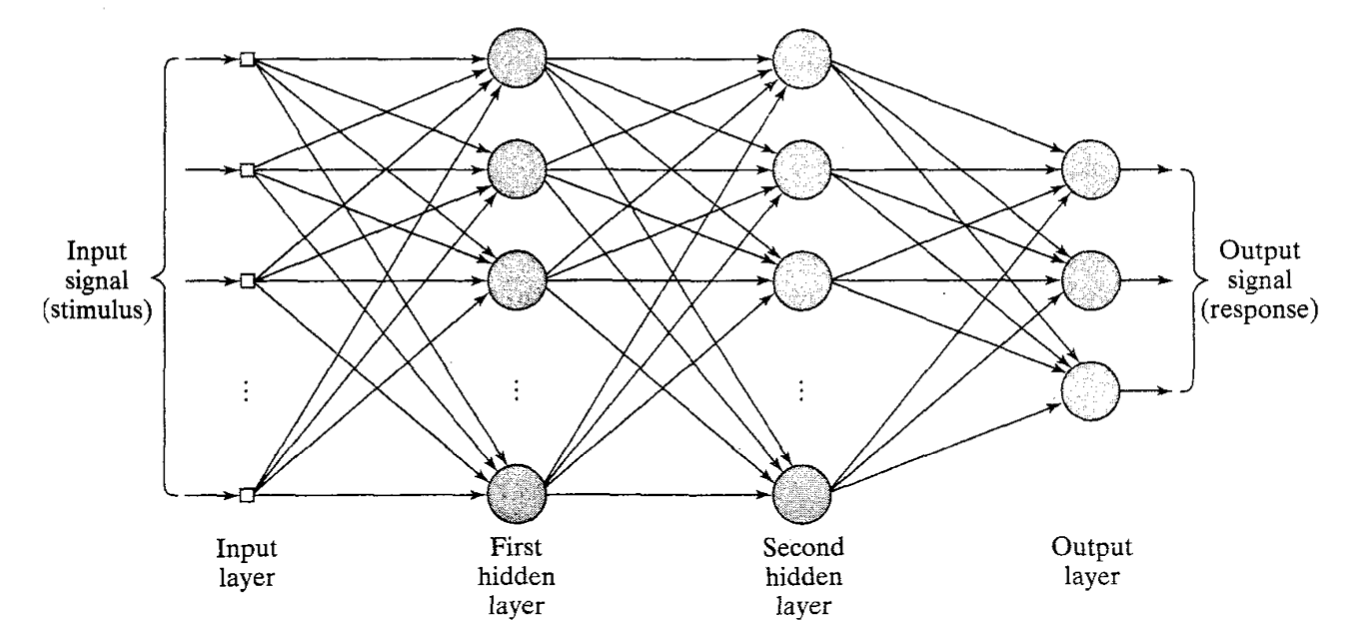
\includegraphics[width=0.65\textwidth]{capitulo2/figuras/an7.png}
	\caption[Grafo arquitectonico de un perceptron multicapa con dos capas ocultas]{Grafo arquitectonico de un perceptron multicapa con dos capas ocultas
		\\\textit{Fuente: Extraído de} \protect\cite[p.281]{haykin1998neural}}
	\label{fig:an7}
\end{figure}

El perceptrón multicapa es una red neuronal típica, puede constar de varias capas y conexiones entre neuronas. Su arquitectura detallada en la figura \ref{fig:an7} sigue la estructura básica de cualquier red neuronal profunda, la misma consta de los siguientes elementos: 
\begin{itemize}

	\item Capa de Entrada: 
	
	Esta capa recibe los datos brutos o características de entrada. Cada neurona en esta capa representa una característica o variable de entrada.

	\item Capas Ocultas: 
	
	Las capas ocultas (una o varias) entre la capa de entrada y la capa de salida procesan los datos y extraen características significativas de manera no lineal. Cada neurona en una capa oculta toma las salidas de la capa anterior como entrada, realiza cálculos y transfiere la salida a la siguiente capa.

	\item Capa de Salida:
	
	Esta capa produce la salida final de la red neuronal. La cantidad de neuronas en esta capa depende del tipo de problema que se esté abordando. Por ejemplo, en un problema de clasificación binaria, podría tener una neurona que produzca una salida entre 0 y 1. En problemas de clasificación multiclase, habría tantas neuronas de salida como clases a predecir, cada una representando la probabilidad de pertenencia a esa clase.
\end{itemize}
\section{APRENDIZAJE AUTOMÁTICO SUPERVISADO}
El aprendizaje automático supervisado, es un enfoque dentro del campo del aprendizaje automático, donde se entrena un modelo utilizando un conjunto de datos etiquetados. En este método, el modelo se entrena para aprender la relación entre las características (variables independientes) y las etiquetas o salidas deseadas (variables dependientes) presentes en los datos de entrenamiento. Como se puede apreciar en la Figura \ref{fig:an8}, donde el conjunto de entrenamiento consiste en mensajes de correo etiquetados como spam o no spam, a partir del cual el modelo podrá predecir a cuál de las dos clases corresponde algún otro correo no etiquetado (nueva instancia). 

\begin{figure}
	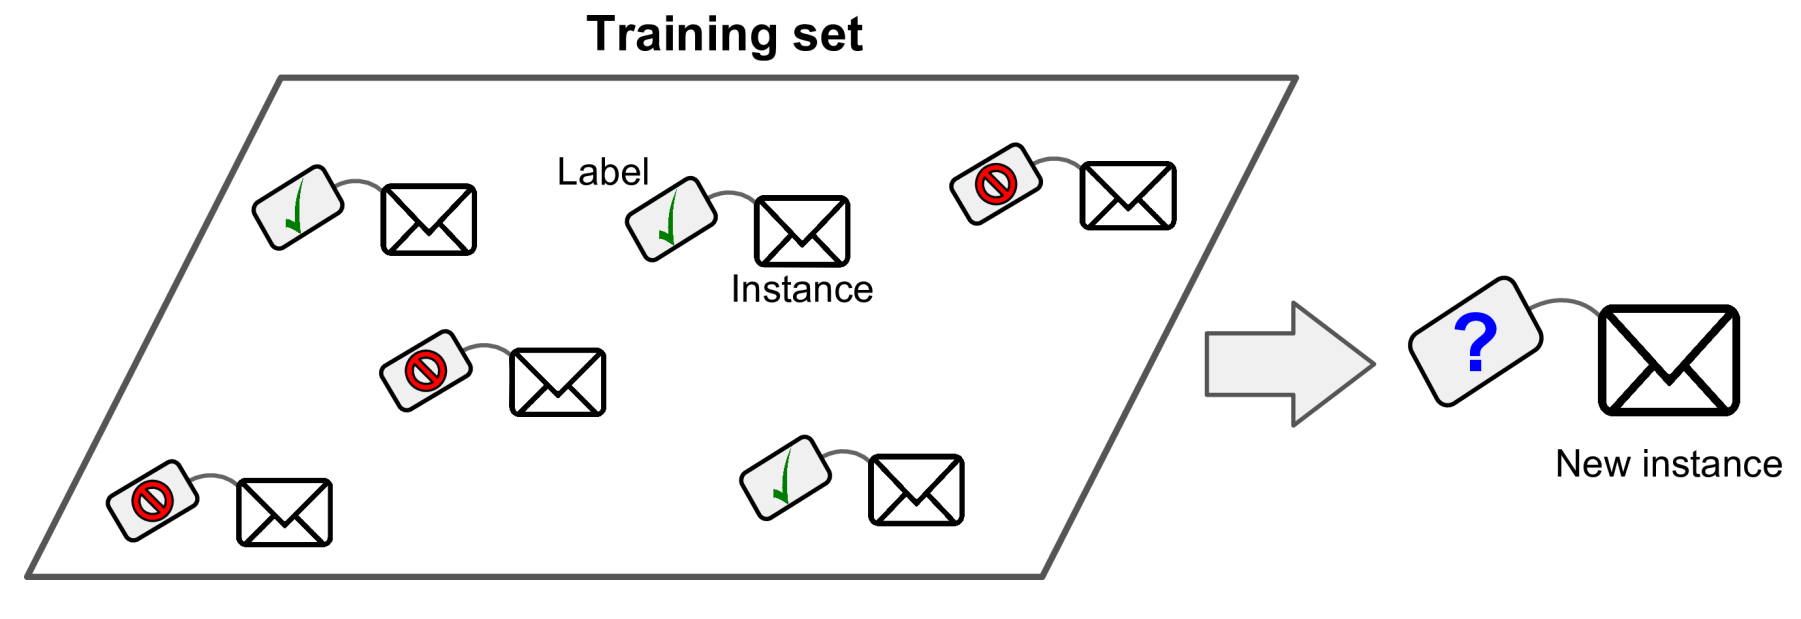
\includegraphics[width=0.65\textwidth]{capitulo2/figuras/an8.png}
	\caption{Un conjunto de entrenamiento etiquetado para aprendizaje supervisado}
	\floatfoot{Fuente: Hands-on machine learning with Scikit-Learn, Keras, and TensorFlow \cite[p. 8]{geron2019hands} }
	\label{fig:an8}
\end{figure}
\subsection{Entrenamiento}
El aprendizaje en una red neuronal supervisada se logra a través de su entrenamiento. Como se mencionó previamente, este proceso implica la adaptación de los pesos y sesgos de las conexiones entre las neuronas para permitir al modelo realizar predicciones precisas sobre nuevos datos. Este proceso se divide en varias fases esenciales que pueden agruparse de la siguiente manera:

\textbf{Propagación hacia adelante}

Una vez que se ha definido la arquitectura de una red neuronal con su cantidad de capas, neuronas por capa, y funciones de activación, el siguiente paso es la inicialización de los pesos. Los pesos y sesgos de la red neuronal pueden ser asignados aleatoriamente o con valores predefinidos.
Lo que sigue es realizar la Propagación hacia Adelante (Forward Propagation) a través de toda la red, este proceso implica el paso de los datos de entrada a través de la red neuronal, capa por capa, desde la capa de entrada hasta la capa de salida, para generar una predicción o salida. Durante esta fase, cada capa de la red neuronal realiza dos operaciones clave:

\begin{itemize}
	\item Ponderación y Suma: Cada neurona en una capa recibe entradas de todas las neuronas de la capa anterior, multiplicadas por los pesos respectivos. Estos productos se suman junto con el sesgo asociado a la neurona. Esta operación puede representarse como $Z=W\cdot X+b$, donde $Z$ almacena el valor de la suma ponderada.
	\item Activación: Después de la suma ponderada, se aplica la función de activación determinada para cada capa a la salida resultante . Esta función introduce no linealidad en la red, permitiendo aprender relaciones y patrones complejos en los datos. Si representamos la función de activación como $A()$, hasta este punto, el proceso realizado sería $A(Z)$, es decir, la suma ponderada pasó por la función de activación. ``Esto da como resultado una cascada directa de cálculos entre las capas, utilizando el conjunto actual de pesos. La salida final prevista se puede comparar con la de la instancia de entrenamiento y se calcula la derivada de la función de pérdida con respecto a la salida.''\cite[p.22]{aggarwal2018neural}.
\end{itemize}

La propagación hacia adelante se utiliza tanto en el entrenamiento como en la predicción de una red neuronal. Durante el entrenamiento, se utiliza para generar predicciones con los datos de entrenamiento y calcular la pérdida, que luego se utiliza en el proceso de retropropagación para ajustar los pesos y mejorar las predicciones. En la predicción o evaluación de nuevos datos, la red simplemente realiza la propagación hacia adelante para generar predicciones sin actualizar los pesos de la red.


\textbf{Propagación hacia atrás}

La retropropagación (backpropagation) en el entrenamiento de redes neuronales ajusta tanto los pesos como los sesgos. Durante el proceso de retropropagación, se calculan los gradientes de la función de coste respecto a todos los pesos y sesgos en la red.

Estos gradientes (derivadas parciales) indican la dirección y la magnitud en la que se debe ajustar cada peso y cada sesgo para minimizar la función de coste. Posteriormente, se utilizan estos gradientes en algoritmos de optimización, como el descenso del gradiente, para actualizar tanto los pesos como los sesgos en la red con el objetivo de mejorar el rendimiento del modelo. Para esto debemos tomar en cuenta los siguientes procedimientos y cálculos a realizar:

\begin{itemize}
	\item Pérdida
	
Una vez que se realiza la primera fase de entrenamiento, obtendremos  la salida correspondiente de la red neuronal, se procederá a calcular la pérdida. La pérdida se calcula con la función de coste, también conocida como función de pérdida, es una métrica que cuantifica qué tan bien está realizando un modelo de aprendizaje automático sus predicciones, al compararlas con las salidas reales o etiquetas conocidas en un conjunto de datos de entrenamiento. 
	\item Función de coste
	
La función de coste, representada como $(C())$, evalúa la discrepancia entre las predicciones del modelo y las salidas esperadas. Esta métrica genera un único valor numérico que indica qué tan distantes se encuentran las predicciones del modelo respecto a las salidas reales. El objetivo primordial es minimizar esta función de coste durante el proceso de entrenamiento con el fin de mejorar las predicciones del modelo.
	
Diversas funciones de coste se emplean según el tipo de problema que se enfrenta. Por ejemplo, en problemas de regresión se utilizan funciones de coste comunes como el error cuadrático medio (mean squared error), el error absoluto medio, el error cuadrático medio logarítmico, entre otros. Para problemas de clasificación, se recurre a la función de pérdida bisagra (hinge loss) en modelos como SVM, y la pérdida focal (focal loss), diseñada para abordar desequilibrios en la distribución de clases.

La selección de la función de coste siempre está ligada al tipo de salida y al problema específico que se está abordando. En todos los casos, existen funciones de coste diseñadas para adaptarse y optimizarse según las necesidades particulares. Por ejemplo, la entropía cruzada suma sobre todas las clases y evalúa la discrepancia entre las distribuciones de probabilidad reales y las predichas para cada clase.
El término $log(y_{i})$ dentro de la entropía cruzada penaliza de manera significativa las predicciones incorrectas o poco confiables. Esta penalización aumenta conforme la predicción se aleja más del valor real. Ver ecuación \ref{eq:e8}

\begin{equation} \label{eq:e8} 
	L(y,{y}')=-\displaystyle\sum_{i=1}^{n}y_{i}log(y_{i}')
\end{equation}


$\sum_{i=1}^{n} =$ sumatoria de todos los valores\\
$y_{i} =$ etiqueta real para la clase i\\
$y_{i}' =$ predicción del modelo para la clase i\\

Esta función de coste se emplea principalmente en problemas de clasificación, abarcando variantes como la entropía cruzada binaria (Binary Cross-Entropy) y la entropía cruzada categórica (Categorical Cross-Entropy).

	\item Vector gradiente
	
	
El siguiente paso implica encontrar las derivadas parciales de todos los parámetros $(w, b)$ de la red neuronal en relación con la función de coste. Este proceso permitirá optimizar la red neuronal utilizando el algoritmo del descenso del gradiente. Para ello, se debe calcular el vector gradiente, el cual consta de las derivadas del costo respecto al peso $\frac{\partial C}{\partial W}$ y las derivadas del costo respecto al sesgo $\frac{\partial C}{\partial b}$.

Hasta este punto, la suma ponderada de cada neurona ha pasado por su respectiva función de activación y finalmente por la función de coste seleccionada, expresada como $C(A(Z))$. Este proceso, donde el resultado de una función se pasa por otra y luego por otra más, se conoce como composición de funciones. Para calcular la derivada de una composición de funciones, se emplea la regla de la cadena (chain rule). Esta regla indica que para encontrar la derivada de una composición de funciones, simplemente se multiplican las derivadas intermedias de cada una. Por ejemplo:

Se tiene dos funciones : $x= h(a) , y= j(c)$

Si existe una relación entre $x$ y $c$ (por ejemplo, $x=2c$), se crea una composición de funciones $x=h(j(c))$, donde $x$ depende de $c$ a través de la función $j$ y luego de $h$.
La regla de la cadena establece que si se tiene una composición de funciones como $x=h(j(c))$, su derivada $\frac{dx}{dc}$ se calcula multiplicando las derivadas de cada función individual.
Es decir, esta derivada es el producto de las derivadas de cada función individual: $\frac{dx}{dc} = \frac{dx}{da} \cdot \frac{da}{dc}$

Por lo tanto hallar la derivada del peso respecto al costo y la derivada del bias respecto al costo de la última capa de la red neuronal equivale a las ecuaciones \ref{eq:e9} y \ref{eq:e10}.
\begin{equation} \label{eq:e9} 
	\frac{\partial C}{\partial W^L}=\frac{\partial C}{\partial A^L}\cdot \frac{\partial A^L }{\partial Z^L}\cdot \frac{\partial Z^L }{\partial W^L}
\end{equation}

\begin{equation} \label{eq:e10} 
	\frac{\partial C}{\partial b^L}=\frac{\partial C}{\partial A^L}\cdot \frac{\partial A^L }{\partial Z^L}\cdot \frac{\partial Z^L }{\partial b^L}
\end{equation}

$\frac{\partial C}{\partial W^L} $.- Representa la derivada parcial de la función de coste C respecto a un peso específico W. Esta derivada indica cómo cambia la función de coste C cuando se modifica un peso particular W en la red.

$\frac{\partial C}{\partial A^L} $.- Es la derivada parcial del coste  respecto a la activación , indica cómo cambia la función de costo C en función de los cambios en la activación A en la última capa L de la red neuronal.

$\frac{\partial A^L }{\partial Z^L} $.- Representa la derivada parcial de la activación A respecto a la suma ponderada Z. Indica cómo pequeños cambios en la suma ponderada Z afectarán la activación A.

$\frac{\partial Z^L }{\partial W^L} $.- Representa la derivada parcial de la suma ponderada Z respecto a un peso particular W, indica como la suma ponderada Z, cambia con respecto a cada peso específico W.

$\frac{\partial C}{\partial b^L} $.- Representa la derivada parcial de la función de coste C respecto al sesgo b. Esta derivada indica cómo cambia la función de coste C cuando se modifica el sesgo b en la red.

$\frac{\partial Z^L }{\partial b^L} $.- Representa la derivada parcial de la suma ponderada Z respecto al sesgo b indica cómo pequeños cambios en el sesgo b afectarán la suma ponderada Z. Sin embargo, es importante tener en cuenta que, la derivada de Z respecto a b generalmente es 1, ya que el sesgo se suma directamente a la suma ponderada Z sin multiplicaciones adicionales.

El cálculo que se realizó hasta ahora es aplicable solamente para la última capa de la red neuronal. La ecuación \ref{eq:e11} y la ecuación \ref{eq:e12} representan las derivadas parciales para la capa $L-1$, es decir la penúltima capa. Estas ecuaciones también son aplicables para todas las capas anteriores. En esta caso  importante notar que las derivadas del coste respecto a la activación $\partial  A^L$  y la derivada de la activación respecto a la suma ponderada  $\frac{\partial  A^L}{\partial  Z^L}$ ya calculadas en la última capa, serán reutilizadas.  Este proceso se repetirá hasta terminar con el cálculo hacia atrás de todas las capas.
\begin{equation} \label{eq:e11} 
	\frac{\partial C}{\partial W^{L-1}}=\frac{\partial C}{\partial A^L}\cdot \frac{\partial A^L }{\partial Z^L}\cdot \frac{\partial Z^L }{\partial A^{L-1}}\cdot \frac{\partial A^{L-1} }{\partial Z^{L-1}}\cdot \frac{\partial Z^{L-1}}{\partial W^{L-1}}
\end{equation}

\begin{equation} \label{eq:e12} 
	\frac{\partial C}{\partial b^{L-1}}=\frac{\partial C}{\partial A^L}\cdot \frac{\partial A^L }{\partial Z^L}\cdot \frac{\partial Z^L }{\partial A^{L-1}}\cdot \frac{\partial A^{L-1} }{\partial Z^{L-1}}\cdot \frac{\partial Z^{L-1}}{\partial b^{L-1}}
\end{equation}


	\item Descenso del gradiente
	
El descenso del gradiente es un algoritmo de optimización cuyo objetivo principal es encontrar el mínimo de una función de coste o pérdida. La idea detrás del descenso del gradiente es iterativamente actualizar los parámetros del modelo (pesos y sesgos ) en la dirección y la magnitud que reduce gradualmente la función de coste. Esto se logra siguiendo el vector del gradiente de la función de coste con respecto a esos parámetros. El gradiente indica la dirección hacia el máximo crecimiento de la función de coste; por lo tanto, avanzar en dirección opuesta al gradiente nos lleva hacia un mínimo local (o global) de la función no convexa. La actualización de los parámetros $\theta$ (pesos, sesgos, etc.) se realiza utilizando la fórmula que se muestra en la ecuación \ref{eq:e13}.
\begin{equation} \label{eq:e13} 
	\theta = \theta - \alpha \cdot\triangledown J(\theta)
\end{equation}


Donde:

$\theta$ son los parámetros del modelo.

$\alpha$  es la tasa de aprendizaje (learning rate), es un valor pequeño que controla la velocidad a la que se actualizan los parámetros.

$\triangledown J(\theta)$  es el gradiente de la función de coste.

El proceso implica utilizar el gradiente de la función de coste con respecto a cada parámetro, y luego ajustar los parámetros en pequeños pasos proporcionales a este gradiente multiplicado por una tasa de aprendizaje (learning rate). Esta tasa de aprendizaje determina la longitud de cada paso que damos hacia el mínimo.

El descenso del gradiente puede tener diferentes variantes, como el descenso del gradiente estocástico (SGD), el descenso del gradiente por lotes (Batch Gradient Descent), el descenso del gradiente en lotes pequeños (Mini Batch Gradient Descent), entre otros, que varían en la cantidad de datos utilizados para cada actualización de los parámetros y la manera en que se actualizan estos parámetros.

\end{itemize}

\subsection{Sobreajuste y Subajuste}
Se detallarán dos conceptos muy importantes que se deben tener en cuenta al momento de examinar el rendimiento de un modelo de aprendizaje automático

\begin{itemize}
\item{Sobreajuste}
\end{itemize}


El sobreajuste (overfitting) es un fenómeno en el aprendizaje automático donde un modelo se ajusta demasiado a los datos de entrenamiento. Esto significa que el modelo aprende no solo los patrones generales presentes en los datos, sino también el ruido o las particularidades específicas de esos datos de entrenamiento. Como resultado, el modelo puede tener un excelente rendimiento en los datos utilizados para entrenarlo pero se desempeña mal al enfrentarse a nuevos datos (conjunto de datos de validación o prueba) que no ha visto antes. Las causas comunes del sobreajuste incluyen:

\begin{itemize}

	\item Modelo demasiado complejo: Un modelo con una capacidad muy alta puede memorizar los datos de entrenamiento en lugar de aprender patrones generales, lo que conduce a un rendimiento deficiente en datos no vistos.
	
	\item Falta de datos: Cuando hay pocos datos disponibles para el entrenamiento, es más probable que el modelo memorice el ruido presente en esos pocos datos en lugar de aprender patrones generales. .``Esta situación es casi similar al aprendizaje de memoria, que es altamente predictivo para los datos de entrenamiento pero no predictivo para los datos de prueba no vistos''\cite[p. 25]{aggarwal2018neural}.
	
	\item Entrenamiento excesivo: Realizar demasiadas iteraciones o épocas de entrenamiento puede llevar a que el modelo se ajuste demasiado a los datos de entrenamiento, perdiendo la capacidad de generalizar.

\end{itemize}

Para evitar el sobreajuste, se pueden utilizar técnicas como la regularización (L1, L2), validación cruzada, reducción de la complejidad del modelo, aumentó de datos, entre otras estrategias.``Una buena regla general es que la cantidad total de puntos de datos de entrenamiento debe ser al menos 2 o 3 veces mayor que la cantidad de parámetros en la red neuronal, aunque la cantidad precisa de instancias de datos depende del modelo específico en cuestión.''\cite[p. 25]{aggarwal2018neural}. Estas técnicas están diseñadas para reducir la capacidad del modelo de ajustarse excesivamente a los datos de entrenamiento y mejorar su capacidad para generalizar a datos no vistos.

\begin{itemize}
\item{Subajuste}
\end{itemize}


El subajuste (underfitting) es un problema en el aprendizaje automático que ocurre cuando un modelo es demasiado simple para capturar la complejidad de los datos. En este caso, el modelo no puede aprender adecuadamente los patrones presentes en los datos de entrenamiento ni en los datos nuevos. Las causas comunes del subajuste incluyen:

\begin{itemize}

	\item Modelo demasiado simple o poca capacidad: Un modelo simple, con pocos parámetros o capas, puede no ser lo suficientemente flexible como para capturar la complejidad de los datos.
	
	\item Falta de características relevantes: Si el conjunto de datos carece de características informativas o si se eliminan características importantes durante el preprocesamiento, el modelo puede ser incapaz de aprender los patrones relevantes.
	
	\item Entrenamiento insuficiente: No entrenar el modelo durante suficientes iteraciones o épocas puede conducir a que el modelo no logre ajustarse adecuadamente a los datos.
	
\end{itemize}

Para abordar el subajuste, se pueden utilizar estrategias como aumentar la complejidad del modelo (añadiendo capas, neuronas, etc.), ajustar los hiperparámetros, mejorar la calidad de los datos o incluso modificar el enfoque del problema. Estas estrategias buscan proporcionar al modelo la capacidad necesaria para aprender patrones más complejos y, por lo tanto, mejorar su rendimiento en los datos de entrenamiento y en la generalización a nuevos datos.

	
\section{REGULARIZACIÓN}
La regularización es una técnica utilizada en el aprendizaje automático para reducir el sobreajuste en modelos, especialmente en aquellos que son propensos a ajustarse demasiado a los datos de entrenamiento.
El objetivo principal de la regularización es agregar cierta penalización a la función de coste o pérdida del modelo para desalentar la complejidad excesiva y, en su lugar, promover modelos más simples que puedan generalizar mejor a datos no vistos. A continuación se detalla métodos de regularización comunes:

\begin{itemize}
	\item L1 (Regularización Lasso): Esta técnica es una versión regularizada de la regresión lineal, se agrega el término de penalización a la función de coste, mismo que  es equivalente a la suma de los valores absolutos de los pesos. Esto puede llevar a algunos pesos a volverse exactamente cero, lo que puede ser útil para la selección automática de características. ``Una característica importante de Lasso Regression es que tiende a eliminar completamente los pesos de las características menos importantes (es decir, establecerlos en cero).''\cite[p. 140]{geron2019hands}. En la ecuación \ref{eq:e14} se observa  El MSE regularizado con L1.
	
	\item L2 (Regularización Ridge): Esta técnica, tiene el efecto de reducir la magnitud de los coeficientes de los parámetros, penalizando los valores grandes y favoreciendo coeficientes más pequeños. Esto ayuda a prevenir el sobreajuste al evitar que los coeficientes crezcan demasiado para adaptarse únicamente a los datos de entrenamiento, es equivalente a la suma de los cuadrados de los pesos. Esto evita que los pesos tomen valores extremadamente grandes y, por lo tanto, controla la complejidad del modelo. ``La regresión de cresta (también llamada regularización de Tikhonov) es una versión regularizada de la regresión lineal: se agrega un término de regularización igual a $ \alpha\sum_{i=1}^{n}  \theta_i^2$ a la función de costo.''\cite[p. 137]{geron2019hands}. En la ecuación \ref{eq:e15} se observa el MSE regularizado con L2
	
\begin{equation} \label{eq:e14} 
	J(\theta) = \text{MSE}(\theta) + \alpha\sum_{i=1}^{n} \left |  \theta_i \right |
\end{equation}

\begin{equation} \label{eq:e15} 
	J(\theta) = \text{MSE}(\theta) + \alpha\frac{1}{2}\sum_{i=1}^{n} \theta_i^2 
\end{equation}									
				
Donde: 
		
		$\alpha $: Es el hiperparámetro de regularización, es decir controla cuánto se desea regularizar el modelo.\\
		$\sum_{i=1}^{n} \left |  \theta_i \right | $:  es la suma de los valores absolutos de los de los parámetros del modelo.\\
		$\sum_{i=1}^{n} \theta_i^2 $: es la suma de los cuadrados de los parámetros del modelo.\\
		
	\item Dropout: Durante el entrenamiento, aleatoriamente se ``apaga'' un conjunto de unidades/neuronas, lo que fuerza a la red a aprender de manera más robusta al evitar la dependencia excesiva de ciertas neuronas.
	
	\item Early Stopping:  La técnica de parada anticipada(early stopping) detiene el entrenamiento de la red antes de que empiece a sobreajustarse. Se basa en monitorear la precisión en un conjunto de validación y detener el entrenamiento cuando la precisión en este conjunto deja de mejorar. ``Una forma muy diferente de regularizar algoritmos de aprendizaje iterativo como el descenso del grandiente es detener el entrenamiento tan pronto como el error de validación alcance un mínimo. A esto se le llama parada anticipada.''\cite[p. 142]{geron2019hands}.
	
\end{itemize}
\section{REDES NEURONALES CONVOLUCIONALES}
Una red neuronal convolucional (CNN) es un tipo de red neuronal artificial que se distingue por incluir una o más capas convolucionales, donde se realiza la operación matemática de convolución. Este tipo de red ha encontrado una amplia aplicación en el campo de la visión artificial. Surgidas de los estudios sobre la corteza visual del cerebro, estas redes han demostrado un éxito notable en el reconocimiento de imágenes.


A pesar de su origen vinculado principalmente al procesamiento visual, las CNN también han mostrado efectividad en la clasificación de documentos. Según \cite{goldberg2016primer} en A Primer on Neural Network Models for Natural Language Processing, las redes neuronales convolucionales son eficaces en la clasificación de documentos porque tienen la capacidad de identificar características sobresalientes (como tokens o secuencias de tokens). Esto resulta útil para tareas de clasificación donde se espera encontrar pistas locales sólidas sobre la pertenencia a una clase, independientemente de que estas pistas puedan presentarse en diversas partes de la entrada. En la Figura \ref{fig:an9} se puede apreciar a una red neuronal convolucional con una matriz bidimensional de tamaño 7x5 donde cada fila representa a cada elemento en la oración de entrada, la tarea de esta red convolucional es extraer frases útiles para realizar una clasificación binaria que indique el sentimiento de la oración de un fragmento de texto.
\begin{figure}[h!]
	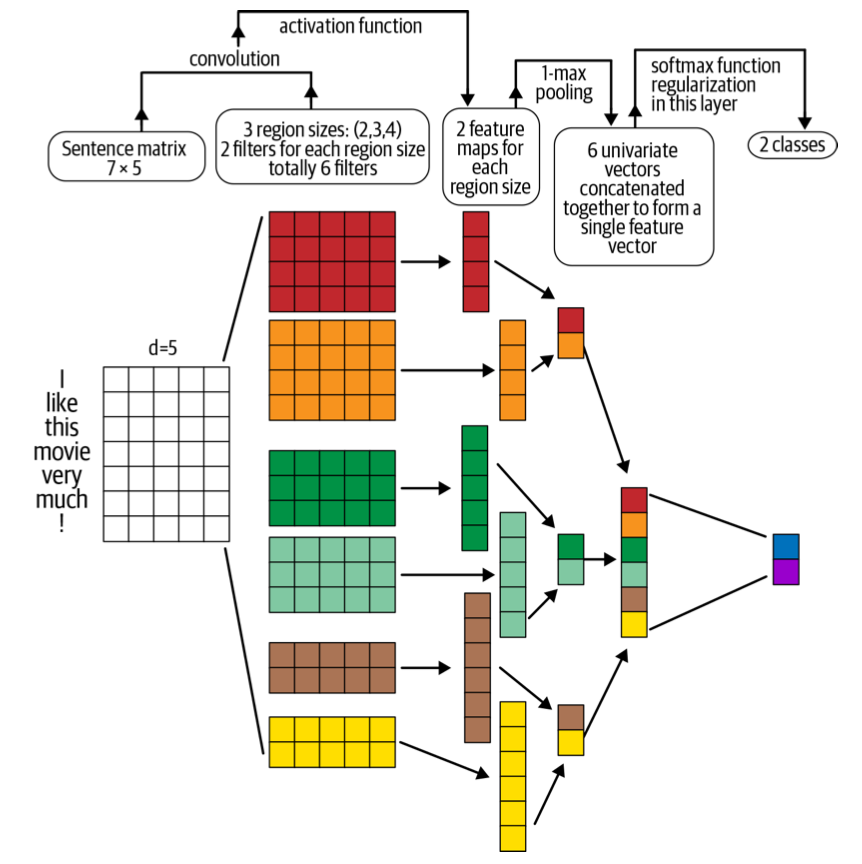
\includegraphics[width=0.6\textwidth]{capitulo2/figuras/an9.png}
	\caption[Modelo CNN en accion]{Modelo CNN en accion
		\\\textit{Fuente: Extraído de} \protect\cite[p. 25]{vajjala2020practical}}
	\label{fig:an9}
\end{figure}

La arquitectura básica de una CNN incluye capas de convolución, las cuales aplican filtros para extraer rasgos relevantes de la entrada. También se incorporan capas de agrupación (pooling) para reducir el tamaño de las representaciones, manteniendo las características más importantes. Por último, las capas totalmente conectadas se encargan de la clasificación final, basándose en los rasgos extraídos por las capas anteriores. Esta arquitectura básica se modifica para adaptarse al procesamiento y clasificación de texto.


\subsection{Breve historia}
Las raíces de las redes neuronales convolucionales (CNN, por sus siglas en inglés Convolutional Neural Networks) se remontan a la década de 1950, cuando entre 1958 y 1959 David Hubel y Torsten Wiesel investigaron la corteza visual realizando experimentos en  gatos. Sus estudios revelaron que muchas de las neuronas en esta región cerebral, tienen pequeños  campos  receptivos locales que reaccionan solamente a estímulos visuales,  ubicados en una región limitada del campo visual.\cite{hubel1959single} Además algunas de estas neuronas  reaccionaban solamente a imágenes con líneas verticales y algunas otras a líneas con distintas orientaciones sin importar que, tuviesen el mismo campo receptivo.  Las neuronas que poseian un campo receptivo más grande, podían reaccionar a patrones más complejos, que eran la combinación de  patrones más simples de un nivel inferior. Este tipo de comportamiento,  hizo que se concluyera a la idea de que las neuronas de nivel superior, se basan en las salidas de las neuronas vecinas de nivel inferior. \cite{hubel1959receptive}

Este trabajo meritorio del Premio Nobel de Fisiología o Medicina inspiró a Fukushima, quien en la década de 1980 propuso la primera arquitectura de red neuronal convolucional conocida como ``Neocognitron''. Este modelo fue capaz de reconocer patrones visuales y estaba compuesto por cuatro tipos de capas entre las cuales resaltaban dos: las capas S (submuestreo) reducían la dimensionalidad de la entrada al tomar secciones de una imagen y reducir su tamaño, preservando las características más relevantes. Las capas C (convolución) eran  responsables de aplicar operaciones de convolución a las entradas. En estas capas, cada neurona estaba conectada únicamente a un área local de las capas previas, reflejando la organización de los campos receptivos locales en las células visuales  \cite{fukushima1980neocognitron}. 

A pesar de estos avances, las CNN no recibieron mayor atención y aplicación práctica hasta la década de 1990, especialmente en el ámbito del reconocimiento de patrones e imágenes. Es en esta época cuando comienzan a destacar y a encontrar aplicaciones prácticas significativas.

El punto de inflexión llegó en 1998, cuando Yann LeCun, junto con otros investigadores, desarrolló una CNN conocida como LeNet-5 para el reconocimiento de dígitos escritos a mano. LeNet-5 fue especialmente revolucionaria porque demostró una alta precisión en la clasificación de dígitos en documentos de cheques bancarios \cite{lecun1998gradient}.

A lo largo de los años, la capacidad de las CNN para procesar datos de imagen se vio fortalecida por la disponibilidad de grandes conjuntos de datos etiquetados, mejoras en hardware (como GPUs) que aceleraron los cálculos intensivos y avances en técnicas de entrenamiento como el uso de funciones de activación no lineales (ReLU) y regularización.

El avance más reciente y significativo de las CNN se produjo con la participación en competiciones de reconocimiento de imágenes, como ImageNet, donde en 2012, un equipo dirigido por Geoffrey Hinton utilizó una CNN denominada ``AlexNet'', que superó ampliamente a otros métodos existentes y estableció un nuevo estándar en el campo de la visión por computadora \cite{krizhevsky2012imagenet}. Desde entonces, las CNN han sido fundamentales en numerosas aplicaciones de reconocimiento de imágenes, segmentación, detección de objetos, entre otros, y continúan siendo objeto de investigación para mejorar su rendimiento y aplicabilidad en una variedad de tareas.

\subsection{Capa de convolución}
La capa de convolución es uno de los componentes fundamentales en una red neuronal convolucional. Esta capa realiza operaciones de convolución en la entrada, lo que permite que la red aprenda características relevantes de los datos, como patrones visuales en una entrada de imágenes.
 \begin{itemize}
\item Filtro
 \end{itemize}


La capa de convolución utiliza filtros (también llamados kernels) que son matrices pequeñas (por ejemplo, 3x3 o 5x5) que se deslizan sobre la entrada. Estos filtros son los parámetros que se aprenden durante el entrenamiento de la red. Durante la fase de entrenamiento, la red aprende automáticamente los valores óptimos para los filtros convolucionales que maximizan su capacidad para reconocer patrones relevantes en los datos de entrada. Este proceso se lleva a cabo de la siguiente manera:
 
 \begin{itemize}
	\item Inicialización de pesos: Al inicio, los pesos de los filtros se inicializan de forma aleatoria o utilizando estrategias específicas.
	
	\item Forward propagation: Durante la fase de forward propagation, los datos se propagan a través de la red. En las capas de convolución, los filtros se aplican a las entradas para generar mapas de características. 
	
	\item Cálculo de la pérdida: Se compara la salida de la red con las etiquetas reales (durante el entrenamiento supervisado) utilizando una función de pérdida, que mide qué tan bien la red está prediciendo las etiquetas.
	
	\item Backpropagation: Utilizando la función de pérdida, se calcula el gradiente de esta función con respecto a los pesos de la red, incluyendo los filtros en las capas de convolución. La retropropagación se utiliza para determinar cómo los pesos deben ajustarse para minimizar la pérdida.
	
	\item Actualización de pesos: Los pesos, incluidos los filtros, se actualizan en la dirección opuesta al gradiente para reducir la pérdida. Se utiliza un algoritmo de optimización, como el descenso de gradiente estocástico (SGD), para realizar estas actualizaciones.

	\item Iteración: Este proceso se repite para múltiples iteraciones (épocas) a medida que la red continúa refinando los pesos y los filtros para mejorar su capacidad de generalización en los datos de entrenamiento.
\end{itemize}

 \begin{itemize}
\item Operación de convolución
 \end{itemize}


En términos generales, la convolución es una operación donde se  aplica un filtro o núcleo a regiones pequeñas de la entrada de la red convolucional, desplazándose secuencialmente. Esto involucra la multiplicación elemento por elemento entre el filtro y la sección correspondiente de la entrada. Estos productos se suman para generar un único valor en una nueva matriz, conocida como mapa de características o feature map, ver Figura \ref{fig:an10}

\begin{figure}[h!]
	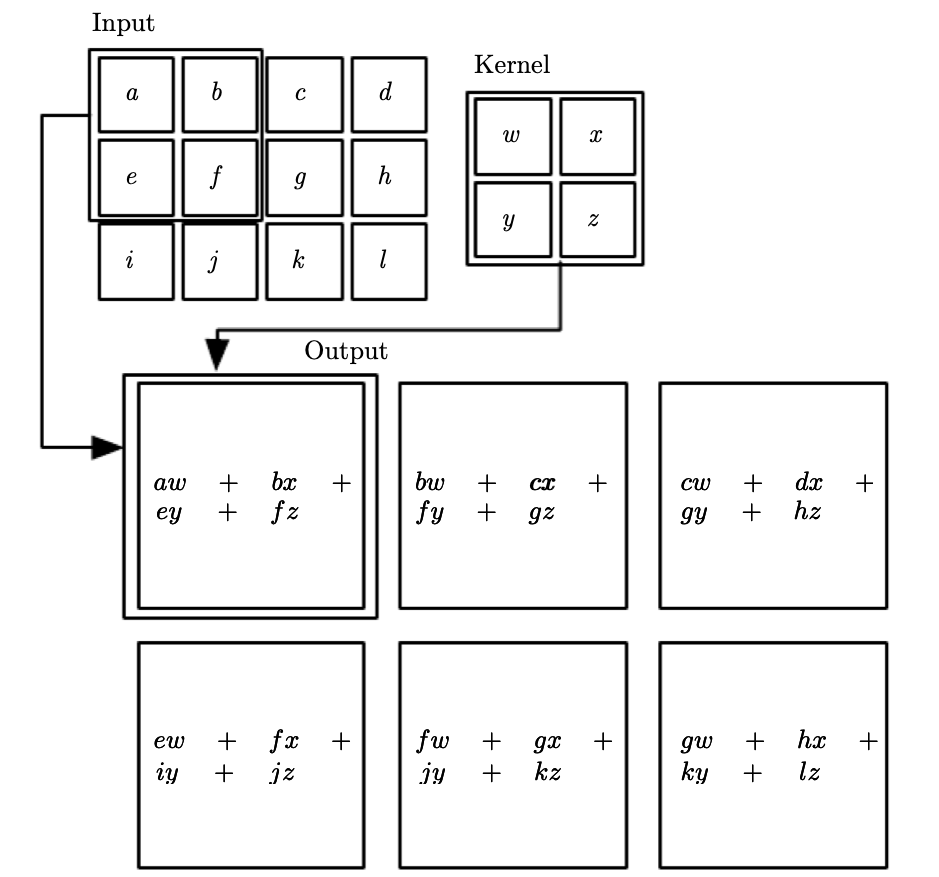
\includegraphics[width=0.6\textwidth]{capitulo2/figuras/an10.png}
	\caption[Convolución valida 2-D sin kernel volteado]{Convolución valida 2-D sin kernel volteado
		\\\textit{Fuente: Extraído de} \protect\cite[p. 334]{goodfellow2016deep}}
	\label{fig:an10}
\end{figure}

Comúnmente, la operación de convolución se representa con un asterisco. ver ecuación \ref{eq:e16}.

\begin{equation} \label{eq:e16} 
	s(i,j)=(I\ast K)
\end{equation}

Por ejemplo, en el caso de que se use un vector bidimensional I como entrada y un núcleo bidimensional K, la operación de convolución sería equivalente a la ecuación \ref{eq:e17} :

\begin{equation} \label{eq:e17} 
	S(i,j)=(I\ast K)(i,j)=\sum_{m}^{}\sum_{n}^{}I(m,n)K(i-m,j-n)
\end{equation}

Si se quiere invertir el núcleo, en el dado caso que se pueda aprovechar la conmutatividad de la operación de convolución, su representación se encuentra en la ecuación \ref{eq:e18}. Donde la  diferencia principal de la ecuación \ref{eq:e17} radica en el orden de los índices de desplazamiento de las variables de la convolución. Ya que a medida que m y n aumentan, los índices de la entrada aumentan, mientras que los de los índices del núcleo disminuyen.

\begin{equation} \label{eq:e18} 
	S(i,j)=(K\ast I)(i,j)=\sum_{m}^{}\sum_{n}^{}I(i-m,j-n)K(m,n)
\end{equation}

Muchas bibliotecas de redes neuronales implementan una función relacionada llamada correlación cruzada como muestra la ecuación \ref{eq:e19}, qué es lo mismo que la convolución pero sin invertir el núcleo.
\begin{equation} \label{eq:e19} 
	(I\ast K)(i,j)=\sum_{m}^{}\sum_{n}^{}I(i+m,j+n)K(m,n)
\end{equation}


La operación de convolución es un paso más para generar el necesario mapa de características, en el caso de que la entrada sea texto se  aplica el filtro w a una ventana de palabras  para crear una nueva característica. Por ejemplo, una característica $c_i$ se genera mediante la mediante la ecuación :

\begin{equation} \label{eq:e20} 
	c_i = f(\mathbf{w}\cdot \mathbf{x}_{i:i+h-1} + b)
\end{equation}
 

	
En la ecuación \ref{eq:e20} $b$ representa el término de sesgo, y $f$ es una función no lineal. El filtro en este caso representado por $w$ se emplea en cada ventana posible de palabras $x_i:i+h-1$ en la oración para generar un mapa de características $c=[c_1,c_2,\ldots,c_{n-h+1}]$. Es decir que, una vez que la entrada pasa por la capa de convolución y se le suma el sesgo, entonces se le aplicará una funcion de activacion para generar salidas no lineales a la entrada para finalmente aplicar la operación de pooling que se detallara más adelante.

 \textbf{Padding}
 
 El padding (relleno) se refiere a agregar valores adicionales alrededor de los bordes de la entrada antes de aplicar el filtro de convolución. Este proceso se utiliza para controlar el tamaño de la salida después de la operación de convolución.
Cuando se aplica un filtro a una entrada en una CNN, el tamaño de la salida se reduce debido a que el filtro no puede aplicarse a los bordes de la entrada. El padding resuelve este problema agregando filas y columnas adicionales de ceros o valores específicos alrededor de la entrada. Estos valores adicionales actúan como un ``borde'' alrededor de la entrada y permiten que el filtro se aplique a las regiones de los bordes de manera más efectiva.

Hay tres tipos comunes de padding: 

\begin{itemize}

	\item Padding ``same'' agrega suficientes filas y columnas de ceros alrededor de la entrada para asegurar que la salida tenga el mismo tamaño que la entrada original después de la convolución. ``En este caso, la red puede contener tantas capas convolucionales como el hardware disponible pueda soportar, ya que la operación de convolución no modifica las posibilidades arquitectónicas disponibles para la siguiente capa.''\cite[p. 350]{goodfellow2016deep}. Sin embargo, los elementos de la entrada cerca del borde influyen en menos elementos de salida que los elementos de la entrada cerca del centro, esto puede hacer que los elementos del borde estén algo subrepresentados en el modelo.
	
	\item Padding ``valid'' no agrega ningún relleno y permite que el filtro se aplique solo a las regiones donde el filtro y la entrada se superponen completamente, lo que produce una salida más pequeña que la entrada. ``Si la imagen de entrada tiene un ancho $m$ y el núcleo tiene un ancho $k$, la salida será de ancho $m - k + 1$. La tasa de esta contracción puede ser dramática si los núcleos utilizados son grandes.'' \cite[p. 350]{goodfellow2016deep}.
	
	\item Padding ``full'' se agregan ceros de tal manera que cada elemento en el borde sea visitado k veces, en cada dirección por el núcleo de convolución. Esto se traduce en una  salida que tiene un ancho mayor  que la entrada original, generalmente $m + k - 1$. En esta configuración, los elementos en los bordes de la  de salida están influenciados por menos elementos de la  entrada que los elementos más cercanos al centro. Esta disparidad puede dificultar que un único núcleo funcione de manera óptima en todas las posiciones del mapa de características.
	
\end{itemize}

El uso de padding en una CNN es crucial para controlar el tamaño de la salida y preservar la información en los bordes de la entrada durante la convolución. Esto es especialmente importante cuando se desean mantener detalles espaciales importantes en la imagen o secuencia de entrada. ``Por lo general, la cantidad óptima de relleno de ceros (en términos de precisión de clasificación del conjunto de pruebas) se encuentra en algún lugar entre la convolución ``válid'' y  ``same''.''\cite[p.350]{goodfellow2016deep}.

\textbf{Stride}

El stride (paso) se refiere a la cantidad de desplazamiento que se aplica al filtro convolucional a medida que se mueve a lo largo de la entrada. Un stride mayor significa que el filtro se mueve en incrementos más grandes, lo que resulta en una reducción del tamaño espacial de la salida. Por otro lado, un stride menor permite un solapamiento más grande entre las operaciones de convolución sucesivas y produce una salida con mayor tamaño espacial.
El ajuste del stride en una CNN puede influir en la dimensionalidad de la salida de cada capa convolucional, lo que a su vez puede afectar el número de parámetros y la información espacial conservada en la red. El stride se elige considerando la complejidad del problema, la dimensionalidad de la entrada y las características que se desean extraer de los datos.


	
\subsection{Capa de agrupación (pooling)}
La capa de agrupación (Pooling Layer) es una etapa crucial que sigue a las capas convolucionales. Su objetivo principal es reducir la dimensionalidad espacial de la representación convolucional, manteniendo las características más importantes.

Hay dos tipos comunes de funciones de agrupación:

\begin{itemize}
	
	\item Max Pooling: Esta función selecciona el valor máximo de una región dentro de la representación convolucional. Ayuda a resaltar las características más relevantes mientras reduce la cantidad de datos y, por ende, el procesamiento necesario.
	
	\item Average Pooling: En esta función, se toma el promedio de los valores dentro de la región seleccionada en lugar de escoger el máximo. Aunque es menos común que Max Pooling, se utiliza para reducir la dimensionalidad manteniendo información general.
	
\end{itemize}

Ambos tipos de funciones de agrupación ayudan a lograr invarianza espacial, lo que significa que la red es capaz de identificar patrones relevantes independientemente de su posición exacta en la imagen o secuencia de entrada.


\subsection{Capa totalmente conectada (fully connected layer)}
El uso de capas totalmente conectadas en una CNN no es obligatorio, depende en gran medida del problema específico y de la arquitectura de la red. Son útiles cuando se necesita combinar y procesar de manera integral las características extraídas por las capas convolucionales y de agrupación para realizar la tarea específica, como la clasificación de imágenes o el procesamiento de texto. Así que después de la extracción de características, se pueden agregar capas densamente conectadas para la clasificación final.

\textbf{Flatten}

La operación de ``flatten'' (aplanado) se refiere a una operación utilizada en redes neuronales para convertir una matriz multidimensional o un tensor en un vector unidimensional. Esta operación toma todas las dimensiones de la entrada y las combina en una única dimensión, conservando todos los elementos pero organizándolos en una única fila.
Después de pasar por varias capas convolucionales y de agrupación (pooling) en la CNN, por ejemplo, se obtiene una salida en forma de tensor tridimensional o multidimensional. Esta salida generalmente se transforma a una forma plana o un vector unidimensional antes de ser alimentada a capas densamente conectadas o totalmente conectadas, ya que las capas densas requieren una entrada en forma de vector unidimensional, para realizar la clasificación final o tareas similares.


\section{DIMENSIONALIDAD}
Por defininir

